\bivtask{Modellierung mit OpenGL}{4}
%
Im Verzeichnis \bivfolder{/home/bildgen/Aufgaben/opengl-1} finden Sie ein 
Rahmenprogramm zu dieser Aufgabe, das die
Initialisierung von \texttt{OpenGL} für Sie übernimmt. Mittels eines 
Aufrufs von \texttt{make} können Sie es kompilieren.

Ergänzen Sie das Zeichnen einer Gruppe von Schneemännern.
Vervollständigen Sie dafür die Funktionen \texttt{drawSnowman} und
\texttt{drawSnowmen}.

Die einzelnen Teile der Schneemänner sollen aus Quadern bestehen.
Dafür existiert bereits eine Funktion namens
\texttt{drawCube(const DrawColour\& col)}, die einen Würfel mit den
Eckpunkten $(-1, -1, -1)$ und $(1, 1, 1)$ sowie der übergebenen Farbe
zeichnet. Mit \texttt{glScalef} und \texttt{glTranslatef} können Sie die
Würfel skalieren und verschieben. Bei der Skalierung kann man für jede 
Koordinatenrichtung einen eigenen Faktor angeben, so dass man den Würfel
in einen Quader transformieren kann. Weiterhin werden Sie die Befehle 
\texttt{glPushMatrix} und \texttt{glPopMatrix} an geeigneten Stellen 
benötigen.

%Eine vollständige Erläuterung des Rahmenprogrammes erhalten Sie in der Übung.
Unten sehen Sie eine Beispielausgabe einer Lösung dieser Aufgabe.

\begin{center}
%   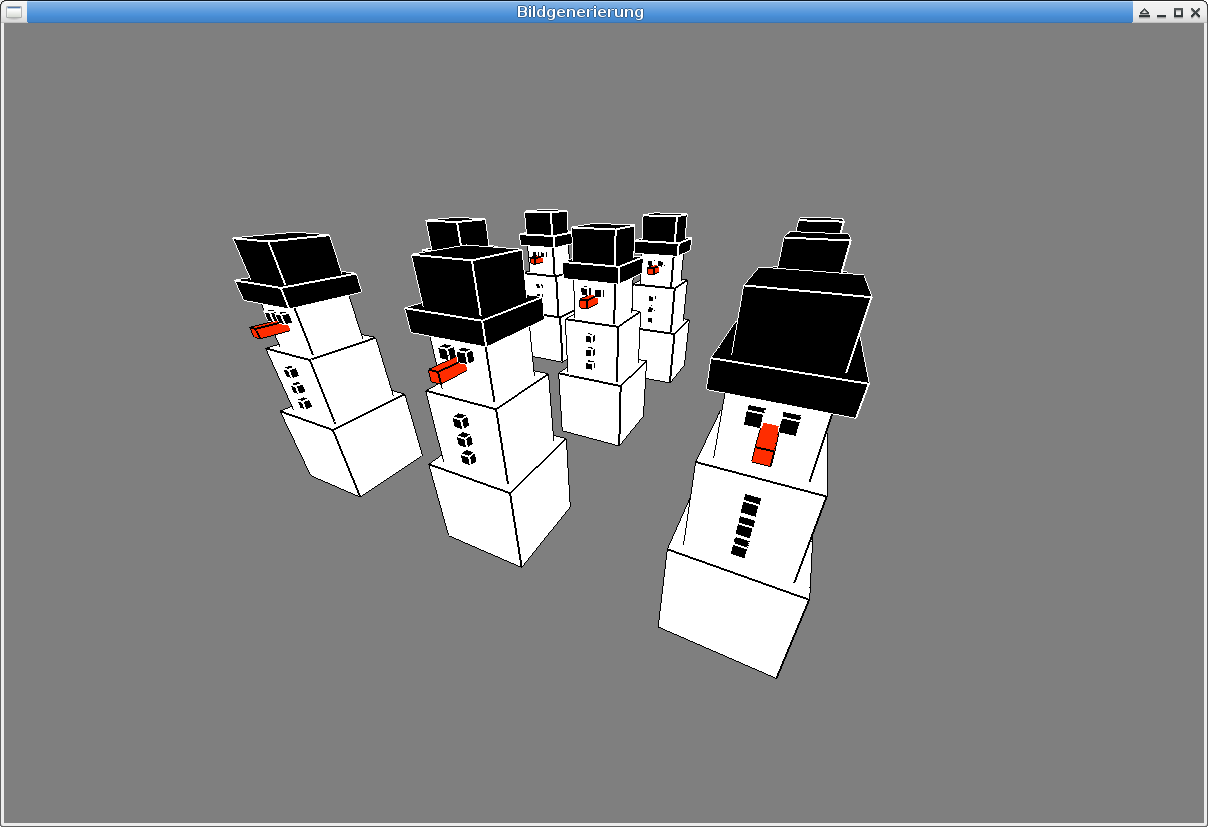
\includegraphics[width=0.7\textwidth]{openglmodellierung.png}
  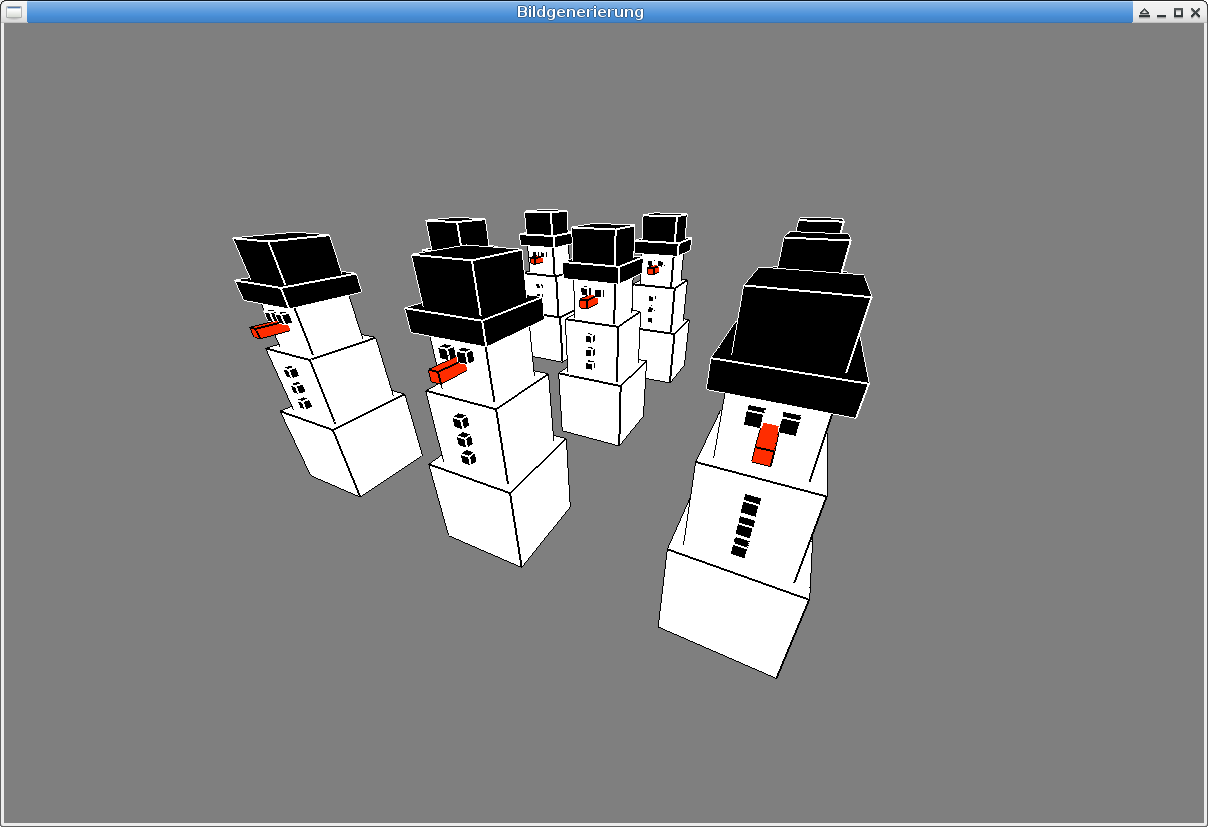
\includegraphics[width=0.5\textwidth]{openglmodellierung.png}
\end{center}
